\documentclass[tikz,border=5pt]{standalone}
\usepackage[T1]{fontenc}
\usepackage{lmodern,amsmath,amssymb}
\usetikzlibrary{arrows.meta,calc,positioning,fit,backgrounds,shapes.geometric,matrix,decorations.pathreplacing,patterns}
\definecolor{ink}{gray}{0.08}
\definecolor{wash}{gray}{0.965}
\definecolor{soft}{gray}{0.45}
\tikzset{box/.style={draw=ink,line width=.65pt,fill=white,align=center,inner sep=4pt,outer sep=0pt,font=\small},flow/.style={draw=ink,line width=.65pt,-{Latex[length=1.8mm,width=1.3mm]},rounded corners=2pt},annotation/.style={font=\scriptsize,text=soft,align=center},groupbox/.style={draw=soft,dashed,line width=.45pt,fill=wash}}
\begin{document}
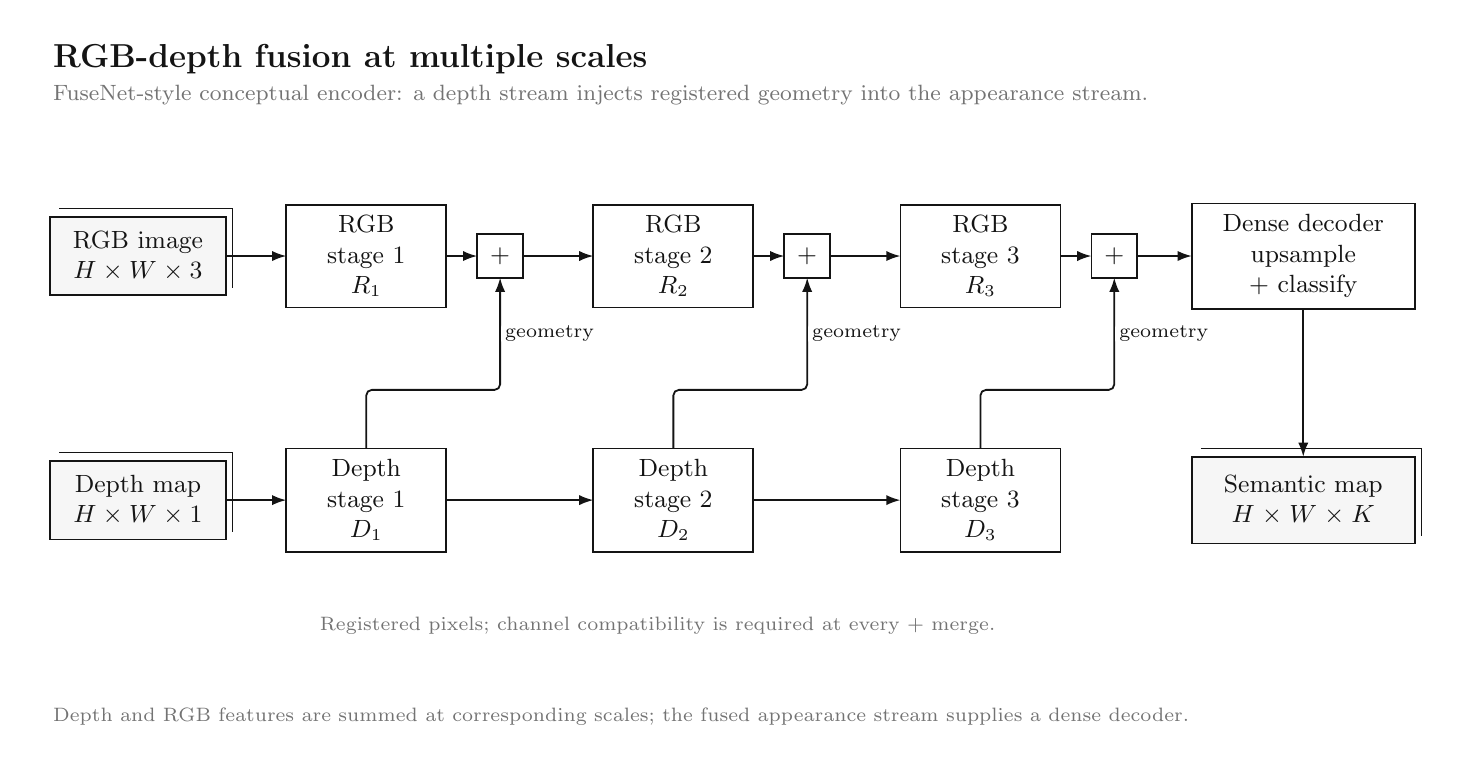
\begin{tikzpicture}[x=1cm,y=-1cm,font=\rmfamily,text=ink]

\path[use as bounding box] (0,0) rectangle (18,9);
\node[anchor=west,font=\large\bfseries] at (.2,.4) {RGB-depth fusion at multiple scales};
\node[anchor=west,font=\footnotesize,text=soft] at (.2,.85) {FuseNet-style conceptual encoder: a depth stream injects registered geometry into the appearance stream.};
\begin{pgfonlayer}{background}
\end{pgfonlayer}
\node[box,fill=wash,minimum width=2.2cm,minimum height=1cm,text width=1.9500000000000002cm] (rgb) at (1.4,2.9) {RGB image\\$H\times W\times3$};
\draw[ink,line width=.4pt] (0.3999999999999998,2.3) -- (2.6,2.3) -- (2.6,3.3);
\node[box,fill=wash,minimum width=2.2cm,minimum height=1cm,text width=1.9500000000000002cm] (depth) at (1.4,6.0) {Depth map\\$H\times W\times1$};
\draw[ink,line width=.4pt] (0.3999999999999998,5.4) -- (2.6,5.4) -- (2.6,6.4);
\node[box,minimum width=2.0cm,minimum height=1.0cm,text width=1.75cm] (r1) at (4.3,2.9) {RGB stage 1\\$R_{1}$};
\node[box,minimum width=2.0cm,minimum height=1.0cm,text width=1.75cm] (d1) at (4.3,6.0) {Depth stage 1\\$D_{1}$};
\node[box,minimum width=0.55cm,minimum height=0.55cm,text width=0.30000000000000004cm] (plus1) at (6.0,2.9) {$+$};
\node[box,minimum width=2.0cm,minimum height=1.0cm,text width=1.75cm] (r2) at (8.2,2.9) {RGB stage 2\\$R_{2}$};
\node[box,minimum width=2.0cm,minimum height=1.0cm,text width=1.75cm] (d2) at (8.2,6.0) {Depth stage 2\\$D_{2}$};
\node[box,minimum width=0.55cm,minimum height=0.55cm,text width=0.30000000000000004cm] (plus2) at (9.899999999999999,2.9) {$+$};
\node[box,minimum width=2.0cm,minimum height=1.0cm,text width=1.75cm] (r3) at (12.1,2.9) {RGB stage 3\\$R_{3}$};
\node[box,minimum width=2.0cm,minimum height=1.0cm,text width=1.75cm] (d3) at (12.1,6.0) {Depth stage 3\\$D_{3}$};
\node[box,minimum width=0.55cm,minimum height=0.55cm,text width=0.30000000000000004cm] (plus3) at (13.799999999999999,2.9) {$+$};
\node[box,minimum width=2.8cm,minimum height=1.1cm,text width=2.55cm] (dec) at (16.2,2.9) {Dense decoder\\upsample + classify};
\node[box,fill=wash,minimum width=2.8cm,minimum height=1.1cm,text width=2.55cm] (seg) at (16.2,6.0) {Semantic map\\$H\times W\times K$};
\draw[ink,line width=.4pt] (14.899999999999999,5.3500000000000005) -- (17.7,5.3500000000000005) -- (17.7,6.45);
\begin{pgfonlayer}{background}
\draw[flow] (r1.east) -- (plus1.west);
\draw[flow] (d1.north) -- (4.3,4.6) -- (6.0,4.6) -- (plus1.south) node[midway,right,fill=white,inner sep=1.5pt,font=\scriptsize] {geometry};
\draw[flow] (r2.east) -- (plus2.west);
\draw[flow] (d2.north) -- (8.2,4.6) -- (9.899999999999999,4.6) -- (plus2.south) node[midway,right,fill=white,inner sep=1.5pt,font=\scriptsize] {geometry};
\draw[flow] (r3.east) -- (plus3.west);
\draw[flow] (d3.north) -- (12.1,4.6) -- (13.799999999999999,4.6) -- (plus3.south) node[midway,right,fill=white,inner sep=1.5pt,font=\scriptsize] {geometry};
\draw[flow] (rgb.east) -- (r1.west);
\draw[flow] (depth.east) -- (d1.west);
\draw[flow] (plus1.east) -- (r2.west);
\draw[flow] (d1.east) -- (d2.west);
\draw[flow] (plus2.east) -- (r3.west);
\draw[flow] (d2.east) -- (d3.west);
\draw[flow] (plus3.east) -- (dec.west);
\draw[flow] (dec.south) -- (seg.north);
\end{pgfonlayer}
\node[annotation,text width=10.5cm] at (8.0,7.6) {Registered pixels; channel compatibility is required at every $+$ merge.};
\node[anchor=west,align=left,font=\scriptsize,text=soft,text width=17.6cm] at (.2,8.75) {Depth and RGB features are summed at corresponding scales; the fused appearance stream supplies a dense decoder.};
\end{tikzpicture}
\end{document}
